In the first test case, as shown in the statement, the fourth segment intersects the first segment at $(0, 1)$.

In the second test case, no two non-consecutive segments intersect:

\begin{center}
  \def \htmlPixelsInCm {45}
  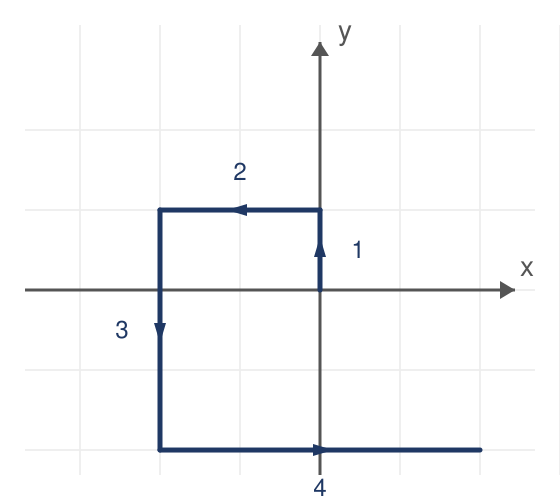
\includegraphics[width=6.5cm]{turtle-t2.svg}
\end{center}

In the third test case, the fourth segment returns to $(0,0)$, which belongs to the first segment, and afterwards the fifth segment (drawn dashed) overlaps the first one entirely:

\begin{center}
  \def \htmlPixelsInCm {45}
  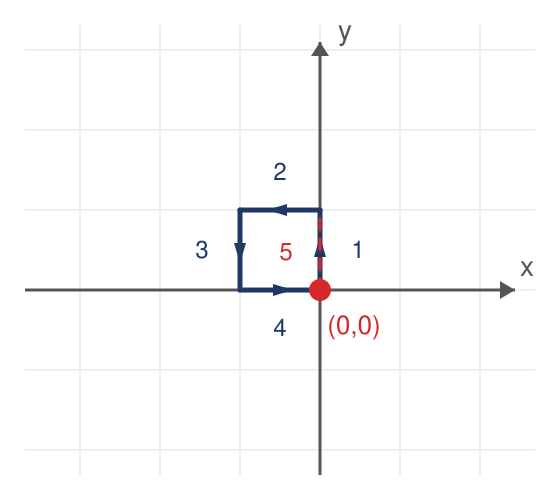
\includegraphics[width=6.5cm]{turtle-t3.svg}
\end{center}
